\section{\ac{SMT}-solvers}

\subsection{School-level system of equations}

I've got this school-level system of equations copypasted from Wikipedia
\footnote{\url{https://en.wikipedia.org/wiki/System_of_linear_equations}}:

\begin{alignat*}{7}
3x &&\; + \;&& 2y             &&\; - \;&& z  &&\; = \;&& 1 & \\
2x &&\; - \;&& 2y             &&\; + \;&& 4z &&\; = \;&& -2 & \\
-x &&\; + \;&& \tfrac{1}{2} y &&\; - \;&& z  &&\; = \;&& 0 &
\end{alignat*}

Will it be possible to solve it using Z3? Here it is:

\begin{lstlisting}
#!/usr/bin/python
from z3 import *

x = Real('x')
y = Real('y')
z = Real('z')
s = Solver()
s.add(3*x + 2*y - z == 1)
s.add(2*x - 2*y + 4*z == -2)
s.add(-x + 0.5*y - z == 0)
print s.check()
print s.model()
\end{lstlisting}

We see this after run:

\begin{lstlisting}
sat
[z = -2, y = -2, x = 1]
\end{lstlisting}

If we change any equation in some way so it will have no solution, s.check() will return ``unsat''.

I've used ``Real'' \textit{sort} (some kind of data type in \ac{SMT}-solvers)
because the last expression equals to $\frac{1}{2}$, which is, of course, a real number.
For the integer system of equations, ``Int'' \textit{sort} would work fine.

Python (and other high-level \ac{PL}s like C\#) interface is highly popular, because it's practical, but in fact, 
there is a standard language for \ac{SMT}-solvers called SMT-LIB
\footnote{\url{http://smtlib.cs.uiowa.edu/papers/smt-lib-reference-v2.5-r2015-06-28.pdf}}.

Our example rewritten to it looks like this:

\begin{lstlisting}
(declare-const x Real)
(declare-const y Real)
(declare-const z Real)
(assert (=(-(+(* 3 x) (* 2 y)) z) 1))
(assert (=(+(-(* 2 x) (* 2 y)) (* 4 z)) -2))
(assert (=(-(+ (- 0 x) (* 0.5 y)) z) 0))
(check-sat)
(get-model)
\end{lstlisting}

This language is very close to LISP, but is somewhat hard to read for untrained eyes.

Now we run it:

\begin{lstlisting}
% z3 -smt2 example.smt
sat
(model
  (define-fun z () Real
    (- 2.0))
  (define-fun y () Real
    (- 2.0))
  (define-fun x () Real
    1.0)
)
\end{lstlisting}

So when you look back to my Python code, you may feel that these 3 expressions could be executed.
This is not true: Z3Py API offers overloaded operators, so expressions are constructed and passed into the guts of Z3 without any execution
\footnote{\url{https://github.com/Z3Prover/z3/blob/6e852762baf568af2aad1e35019fdf41189e4e12/src/api/python/z3.py}}.
I would call it ``embedded \ac{DSL}''.

Same thing for Z3 C++ API, you may find there ``operator+'' declarations and many more
\footnote{\url{https://github.com/Z3Prover/z3/blob/6e852762baf568af2aad1e35019fdf41189e4e12/src/api/c\%2B\%2B/z3\%2B\%2B.h}}.

Z3 \ac{API}s for Java, ML and .NET are also exist
\footnote{\url{https://github.com/Z3Prover/z3/tree/6e852762baf568af2aad1e35019fdf41189e4e12/src/api}}.\\
\\
Z3Py tutorial: \url{https://github.com/ericpony/z3py-tutorial}.

Z3 tutorial which uses SMT-LIB language: \url{http://rise4fun.com/Z3/tutorial/guide}.

\subsection{Another school-level system of equations}
\label{eq2_SMT}

I've found this somewhere at Facebook:

\begin{figure}[H]
\centering
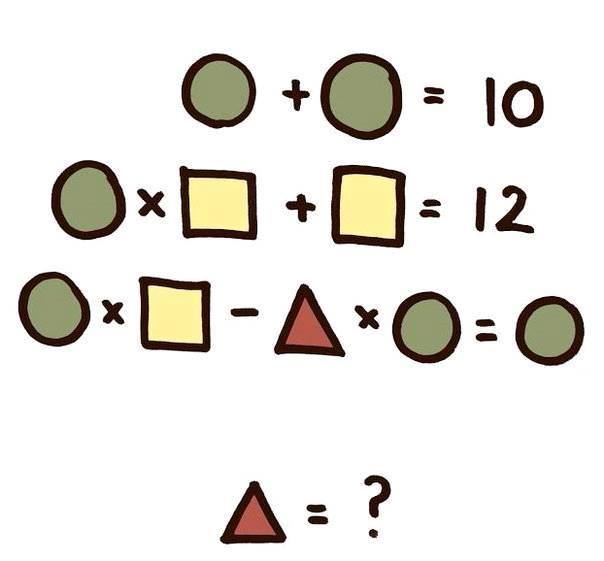
\includegraphics[scale=0.3]{SMT/equation.jpg}
\caption{System of equations}
\end{figure}

It's that easy to solve it in Z3:

\begin{lstlisting}
#!/usr/bin/python
from z3 import *

circle, square, triangle = Ints('circle square triangle')
s = Solver()
s.add(circle+circle==10)
s.add(circle*square+square==12)
s.add(circle*square-triangle*circle==circle)
print s.check()
print s.model()
\end{lstlisting}

\begin{lstlisting}
sat
[triangle = 1, square = 2, circle = 5]
\end{lstlisting}

\subsection{Connection between \ac{SAT} and \ac{SMT} solvers}

\ac{SMT}-solvers are frontends to \ac{SAT} solvers, i.e.,
they translating input SMT expressions into \ac{CNF} and feed SAT-solver with it.
Translation process is sometimes called ``bit blasting''.
Some \ac{SMT}-solvers uses external SAT-solver: STP uses MiniSAT or CryptoMiniSAT as backend.
Some other \ac{SMT}-solvers (like Z3) has their own SAT solver.

% subsections
\subsection{Generating de Bruijn sequences using Z3}

The following piece of quite esoteric code calculates number of leading zero bits
\footnote{\url{https://en.wikipedia.org/wiki/Find_first_set}}:

\begin{lstlisting}
int v[64]=
	{ -1,31, 8,30, -1, 7,-1,-1, 29,-1,26, 6, -1,-1, 2,-1,
	  -1,28,-1,-1, -1,19,25,-1, 5,-1,17,-1, 23,14, 1,-1,
	   9,-1,-1,-1, 27,-1, 3,-1, -1,-1,20,-1, 18,24,15,10,
	  -1,-1, 4,-1, 21,-1,16,11, -1,22,-1,12, 13,-1, 0,-1 };

int LZCNT(uint32_t x)
{
    x |= x >> 1;
    x |= x >> 2;
    x |= x >> 4;
    x |= x >> 8;
    x |= x >> 16;
    x *= 0x4badf0d;
    return v[x >> 26];
}
\end{lstlisting}

(This is usually done using simpler algorithm, but it will contain conditional jumps, which is bad for
CPUs starting at RISC. There are no conditional jumps in this algorithm.)

Read more about it: \url{https://yurichev.com/blog/de_bruijn/}.
The magic number used here is called \textit{de Bruijn sequence},
and I once used bruteforce to find it (one of the results was \textit{0x4badf0d}, which is used here).
But what if we need magic number for 64-bit values?
Bruteforce is not an option here.

If you already read about these sequences in my blog or in other sources,
you can see that the 32-bit magic number is a number consisting
of 5-bit overlapping chunks, and all chunks must be unique, i.e., must not be repeating.

For 64-bit magic number, these are 6-bit overlapping chunks.

To find the magic number, one can find a Hamiltonian path of a de Bruijn graph.
But I've found that Z3 is also can do this, though, overkill, but this is more illustrative.

\lstinputlisting{SMT/de_bruijn/64.py}

We just enumerate all overlapping 6-bit chunks and tell Z3 that they must be unique (see \TT{Distinct}).
Output:

\lstinputlisting{SMT/de_bruijn/output.txt}

Overlapping chunks are clearly visible.
So the magic number is \textit{0x79c52dd0991abf60}.
Let's check:

\lstinputlisting{SMT/de_bruijn/64.c}

That works!

More about de Bruijn sequences:
\url{https://yurichev.com/blog/de_bruijn/},
\url{https://chessprogramming.wikispaces.com/De+Bruijn+sequence},
\url{https://chessprogramming.wikispaces.com/De+Bruijn+Sequence+Generator}.


\subsection{Zebra puzzle (\ac{AKA} Einstein puzzle)}
\label{zebra_SMT}

Zebra puzzle is a popular puzzle, defined as follows:

% FIXME remove paragraph at first line
\begin{framed}
\begin{quotation}
1.There are five houses.\\
2.The Englishman lives in the red house.\\
3.The Spaniard owns the dog.\\
4.Coffee is drunk in the green house.\\
5.The Ukrainian drinks tea.\\
6.The green house is immediately to the right of the ivory house.\\
7.The Old Gold smoker owns snails.\\
8.Kools are smoked in the yellow house.\\
9.Milk is drunk in the middle house.\\
10.The Norwegian lives in the first house.\\
11.The man who smokes Chesterfields lives in the house next to the man with the fox.\\
12.Kools are smoked in the house next to the house where the horse is kept.\\
13.The Lucky Strike smoker drinks orange juice.\\
14.The Japanese smokes Parliaments.\\
15.The Norwegian lives next to the blue house.\\
\\
Now, who drinks water? Who owns the zebra?\\
\\
In the interest of clarity, it must be added that each of the five houses is painted a different color, and their inhabitants are of different national extractions, own different pets, drink different beverages and smoke different brands of American cigarets [sic]. One other thing: in statement 6, right means your right.
\end{quotation}
\end{framed}
( \url{https://en.wikipedia.org/wiki/Zebra_Puzzle} ) \\
\\
It's a very good example of \ac{CSP}.

We would encode each entity as integer variable, representing number of house.

Then, to define that Englishman lives in red house, we will add this constraint: \TT{Englishman == Red}, meaning that number of a house where Englishmen resides and which is painted in red is the same.

To define that Norwegian lives next to the blue house, we don't realy know, if it is at left side of blue house or at right side, but we know that house numbers are different by just 1.
So we will define this constraint: \TT{Norwegian==Blue-1 OR Norwegian==Blue+1}.

We will also need to limit all house numbers, so they will be in range of 1..5.

We will also use \TT{Distinct} to show that all various entities of the same type are all has different house numbers.

\lstinputlisting{SMT/zebra.py}

When we run it, we got correct result:

\begin{lstlisting}
sat
[Snails = 3,
 Blue = 2,
 Ivory = 4,
 OrangeJuice = 4,
 Parliament = 5,
 Yellow = 1,
 Fox = 1,
 Zebra = 5,
 Horse = 2,
 Dog = 4,
 Tea = 2,
 Water = 1,
 Chesterfield = 2,
 Red = 3,
 Japanese = 5,
 LuckyStrike = 4,
 Norwegian = 1,
 Milk = 3,
 Kools = 1,
 OldGold = 3,
 Ukrainian = 2,
 Coffee = 5,
 Green = 5,
 Spaniard = 4,
 Englishman = 3]
 \end{lstlisting}


\subsection{Sudoku puzzle}
\label{sudoku_SMT}

Sudoku puzzle is a 9*9 grid with some cells filled with values, some are empty:

% copypasted from http://www.texample.net/tikz/examples/sudoku/
\newcounter{row}
\newcounter{col}

\newcommand\setrow[9]{
  \setcounter{col}{1}
  \foreach \n in {#1, #2, #3, #4, #5, #6, #7, #8, #9} {
    \edef\x{\value{col} - 0.5}
    \edef\y{9.5 - \value{row}}
    \node[anchor=center] at (\x, \y) {\n};
    \stepcounter{col}
  }
  \stepcounter{row}
}

\begin{center}
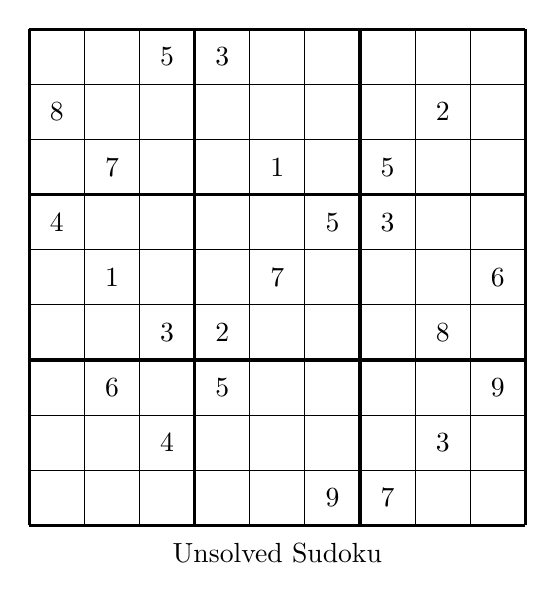
\begin{tikzpicture}[scale=.7]
  \begin{scope}
    \draw (0, 0) grid (9, 9);
    \draw[very thick, scale=3] (0, 0) grid (3, 3);

    \setcounter{row}{1}
    \setrow { }{ }{5}  {3}{ }{ }  { }{ }{ }
    \setrow {8}{ }{ }  { }{ }{ }  { }{2}{ }
    \setrow { }{7}{ }  { }{1}{ }  {5}{ }{ }

    \setrow {4}{ }{ }  { }{ }{5}  {3}{ }{ }
    \setrow { }{1}{ }  { }{7}{ }  { }{ }{6}
    \setrow { }{ }{3}  {2}{ }{ }  { }{8}{ }

    \setrow { }{6}{ }  {5}{ }{ }  { }{ }{9}
    \setrow { }{ }{4}  { }{ }{ }  { }{3}{ }
    \setrow { }{ }{ }  { }{ }{9}  {7}{ }{ }

    \node[anchor=center] at (4.5, -0.5) {Unsolved Sudoku};
  \end{scope}
\end{tikzpicture}
\end{center}

Numbers of each row must be unique, i.e., it must contain all 9 numbers in range of 1..9 without repetition.
Same story for each column and also for each 3*3 square.

This puzzle is good candidate to try \ac{SMT} solver on, because it's essentially an unsolved system of equations.

\subsubsection{The first idea}

The only thing we must decide is that how to determine in one expression, if the input 9 variables has all 9 unique numbers?
They are not ordered or sorted, after all.

From the school-level arithmetics, we can devise this idea:

\begin{equation}
\underbrace{10^{i_1} + 10^{i_2} + \cdots + 10^{i_9}}_9 = 1111111110
\end{equation}

Take each input variable, calculate $10^i$ and sum them all.
If all input values are unique, each will be settled at its own place.
Even more than that: there will be no holes, i.e., no skipped values.
So, in case of Sudoku, 1111111110 number will be final result, indicating that all 9 input values are unique, in range of 1..9.

Exponentiation is heavy operation, can we use binary operations? Yes, just replace 10 with 2:

\begin{equation}
\underbrace{2^{i_1} + 2^{i_2} + \cdots + 2^{i_9}}_9 = 1111111110_2
\end{equation}

The effect is just the same, but the final value is in base 2 instead of 10.

Now a working example:

\lstinputlisting{SMT/sudoku_plus.py}
( \url{https://github.com/dennis714/SAT_SMT_article/blob/master/SMT/sudoku_plus.py} )

\begin{lstlisting}
% time python sudoku_plus.py
1 4 5 3 2 7 6 9 8
8 3 9 6 5 4 1 2 7
6 7 2 9 1 8 5 4 3
4 9 6 1 8 5 3 7 2
2 1 8 4 7 3 9 5 6
7 5 3 2 9 6 4 8 1
3 6 7 5 4 2 8 1 9
9 8 4 7 6 1 2 3 5
5 2 1 8 3 9 7 6 4

real    0m11.717s
user    0m10.896s
sys     0m0.068s
\end{lstlisting}

Even more, we can replace summing operation to logical OR:

\begin{equation}
\underbrace{2^{i_1} \vee 2^{i_2} \vee \cdots \vee 2^{i_9}}_9 = 1111111110_2
\end{equation}

% FIXME: только часть исходника
\lstinputlisting{SMT/sudoku_or.py}
( \url{https://github.com/dennis714/SAT_SMT_article/blob/master/SMT/sudoku_or.py} )

Now it works much faster. Z3 handles OR operation over bit vectors better than addition?

\begin{lstlisting}
% time python sudoku_or.py
1 4 5 3 2 7 6 9 8
8 3 9 6 5 4 1 2 7
6 7 2 9 1 8 5 4 3
4 9 6 1 8 5 3 7 2
2 1 8 4 7 3 9 5 6
7 5 3 2 9 6 4 8 1
3 6 7 5 4 2 8 1 9
9 8 4 7 6 1 2 3 5
5 2 1 8 3 9 7 6 4

real    0m1.429s
user    0m1.393s
sys     0m0.036s
\end{lstlisting}

The puzzle I used as example is dubbed as one of the hardest known
\footnote{\url{http://www.mirror.co.uk/news/weird-news/worlds-hardest-sudoku-can-you-242294}} (well, for humans).
It took $\approx 1.4$ seconds on my Intel Core i3-3110M 2.4GHz notebook to solve it.

\subsubsection{The second idea}

My first approach is far from effective, I did what first came to my mind and worked.
Another approach is to use \TT{distinct} command from SMT-LIB, which tells Z3 that some variables must be distinct (or unique).
This command is also available in Z3 Python interface.

I've rewritten my first Sudoku solver, now it operates over \textit{Int} \textit{sort}, it has \TT{distinct} commands instead of bit operations,
and now also other constaint added: each cell value must be in 1..9 range, because, otherwise, Z3 will offer (although correct) solution with too big
and/or negative numbers.

% FIXME: только часть исходника
\lstinputlisting{SMT/sudoku2.py}
( \url{https://github.com/dennis714/SAT_SMT_article/blob/master/SMT/sudoku2.py} )

\begin{lstlisting}
% time python sudoku2.py
1 4 5 3 2 7 6 9 8
8 3 9 6 5 4 1 2 7
6 7 2 9 1 8 5 4 3
4 9 6 1 8 5 3 7 2
2 1 8 4 7 3 9 5 6
7 5 3 2 9 6 4 8 1
3 6 7 5 4 2 8 1 9
9 8 4 7 6 1 2 3 5
5 2 1 8 3 9 7 6 4

real    0m0.382s
user    0m0.346s
sys     0m0.036s
\end{lstlisting}

That's much faster.

\subsubsection{Conclusion}

\ac{SMT}-solvers are so helpful, is that our Sudoku solver has nothing else, we have just defined relationships between variables (cells).

\subsubsection{Homework}

As it seems, true Sudoku puzzle is the one which has only one solution.
The piece of code I've included here shows only the first one.
Using the method described earlier (\ref{SMTEnumerate}, also called ``model counting''), 
try to find more solutions, or prove that the solution you have just found is the only one possible.

\subsubsection{Further reading}

\url{http://www.norvig.com/sudoku.html}

\subsubsection{Sudoku as a \ac{SAT} problem}

It's also possible to represend Sudoku puzzle as a huge \ac{CNF} equation and use \ac{SAT}-solver to find solution, but it's just trickier.

Some articles about it:
\textit{Building a Sudoku Solver with SAT}\footnote{\url{http://ocw.mit.edu/courses/electrical-engineering-and-computer-science/6-005-elements-of-software-construction-fall-2011/assignments/MIT6_005F11_ps4.pdf}},
Tjark Weber, \textit{A SAT-based Sudoku Solver}\footnote{\url{https://www.lri.fr/~conchon/mpri/weber.pdf}},
Ines Lynce, Joel Ouaknine, \textit{Sudoku as a SAT Problem}\footnote{\url{http://sat.inesc-id.pt/~ines/publications/aimath06.pdf}},
Gihwon Kwon, Himanshu Jain, \textit{Optimized CNF Encoding for Sudoku Puzzles}\footnote{\url{http://www.cs.cmu.edu/~hjain/papers/sudoku-as-SAT.pdf}}.

\ac{SMT}-solver can also use \ac{SAT}-solver in its core, so it does all mundane translating work.
As a ``compiler'', it may not do this in the most efficient way, though.


\subsection{Solving Problem Euler 31: ``Coin sums''}

(This text was first published in my blog\footnote{\url{http://dennisyurichev.blogspot.de/2013/05/in-england-currency-is-made-up-of-pound.html}} at 10-May-2013.)

\begin{framed}
\begin{quotation}
In England the currency is made up of pound, £, and pence, p, and there are eight coins in general circulation:

1p, 2p, 5p, 10p, 20p, 50p, £1 (100p) and £2 (200p).
It is possible to make £2 in the following way:

1£1 + 150p + 220p + 15p + 12p + 31p
How many different ways can £2 be made using any number of coins?
\end{quotation}
\end{framed}
( \href{http://projecteuler.net/problem=31}{Problem Euler 31 --- Coin sums} )

\label{SMTEnumerate}
Using Z3 for solving this is overkill, and also slow, but nevertheless, it works, showing all possible solutions as well.
The piece of code for blocking already found solution and search for next, and thus, counting all solutions, was taken from Stack Overflow answer
\footnote{\url{http://stackoverflow.com/questions/11867611/z3py-checking-all-solutions-for-equation}, 
another question: \url{http://stackoverflow.com/questions/13395391/z3-finding-all-satisfying-models}}.
This is also called ``model counting''.
Constraints like ``a>=0'' must be present, because Z3 solver will find solutions with negative numbers.

\begin{lstlisting}
#!/usr/bin/python

from z3 import *

a,b,c,d,e,f,g,h = Ints('a b c d e f g h')
s = Solver()
s.add(1*a + 2*b + 5*c + 10*d + 20*e + 50*f + 100*g + 200*h == 200, 
   a>=0, b>=0, c>=0, d>=0, e>=0, f>=0, g>=0, h>=0)
result=[]

while True:
    if s.check() == sat:
        m = s.model()
        print m
        result.append(m)
        # Create a new constraint the blocks the current model
        block = []
        for d in m:
            # d is a declaration
            if d.arity() > 0:
                raise Z3Exception("uninterpreted functions are not suppported")
            # create a constant from declaration
            c=d()
            #print c, m[d]
            if is_array(c) or c.sort().kind() == Z3_UNINTERPRETED_SORT:
                raise Z3Exception("arrays and uninterpreted sorts are not supported")
            block.append(c != m[d])
        #print "new constraint:",block
        s.add(Or(block))
    else:
        print len(result)
        break
\end{lstlisting}

Works very slow, and this is what it produces:

\begin{lstlisting}
[h = 0, g = 0, f = 0, e = 0, d = 0, c = 0, b = 0, a = 200]
[f = 1, b = 5, a = 0, d = 1, g = 1, h = 0, c = 2, e = 1]
[f = 0, b = 1, a = 153, d = 0, g = 0, h = 0, c = 1, e = 2]
...
[f = 0, b = 31, a = 33, d = 2, g = 0, h = 0, c = 17, e = 0]
[f = 0, b = 30, a = 35, d = 2, g = 0, h = 0, c = 17, e = 0]
[f = 0, b = 5, a = 50, d = 2, g = 0, h = 0, c = 24, e = 0]
\end{lstlisting}

73682 results in total.

\subsection{Using Z3 theorem prover to prove equivalence of some weird alternative to XOR operation}
\label{weird_XOR}

(The test was first published in my blog at April 2015: \url{http://blog.yurichev.com/node/86}).

There is a ``A Hacker's Assistant'' program\footnote{\url{http://www.hackersdelight.org/}} (\textit{Aha!}) written by Henry Warren,
who is also the author of the great ``Hacker's Delight'' book.

The \textit{Aha!} program is essentially \textit{superoptimizer}\footnote{\url{http://en.wikipedia.org/wiki/Superoptimization}},
which blindly brute-force a list of some generic RISC CPU instructions to achieve shortest possible (and jumpless or branch-free) 
CPU code sequence for desired operation.
For example, \textit{Aha!} can find jumpless version of abs() function easily.

Compiler developers use superoptimization to find shortest possible (and/or jumpless) code,
but I tried to do otherwise---to find longest code for some primitive operation.
I tried \textit{Aha!} to find equivalent of basic XOR operation without usage of the actual XOR instruction,
and the most bizarre example \textit{Aha!} gave is:

\begin{lstlisting}
Found a 4-operation program:
   add   r1,ry,rx
   and   r2,ry,rx
   mul   r3,r2,-2
   add   r4,r3,r1
   Expr: (((y & x)*-2) + (y + x))
\end{lstlisting}

And it's hard to say, why/where we can use it, maybe for obfuscation, I'm not sure.
I would call this \textit{suboptimization} (as opposed to \textit{superoptimization}).
Or maybe \textit{superdeoptimization}.

But my another question was also, is it possible to prove that this is correct formula at all?
The \textit{Aha!} checking some intput/output values against XOR operation, but of course, not all the possible values.
It is 32-bit code, so it may take very long time to try all possible 32-bit inputs to test it.

We can try Z3 theorem prover for the job. It's called \textit{prover}, after all.

So I wrote this:

\begin{lstlisting}
#!/usr/bin/python
from z3 import *

x = BitVec('x', 32)
y = BitVec('y', 32)
output = BitVec('output', 32)
s = Solver()
s.add(x^y==output)
s.add(((y & x)*0xFFFFFFFE) + (y + x)!=output)
print s.check()
\end{lstlisting}

In plain English language, this means
``are there any case for $x$ and $y$ where $x \oplus y$ doesn't equals to $((y \& x)*-2) + (y + x)$?''
\dots and Z3 prints ``unsat'', meaning, it can't find any counterexample to the equation.
So this \textit{Aha!} result is proved to be working just like XOR operation.

Oh, I also tried to extend the formula to 64 bit:

\begin{lstlisting}
#!/usr/bin/python
from z3 import *

x = BitVec('x', 64)
y = BitVec('y', 64)
output = BitVec('output', 64)
s = Solver()
s.add(x^y==output)
s.add(((y & x)*0xFFFFFFFE) + (y + x)!=output)
print s.check()
\end{lstlisting}

Nope, now it says ``sat'', meaning, Z3 found at least one counterexample.
Oops, it's because I forgot to extend -2 number to 64-bit value:

\begin{lstlisting}
#!/usr/bin/python
from z3 import *

x = BitVec('x', 64)
y = BitVec('y', 64)
output = BitVec('output', 64)
s = Solver()
s.add(x^y==output)
s.add(((y & x)*0xFFFFFFFFFFFFFFFE) + (y + x)!=output)
print s.check()
\end{lstlisting}

Now it says ``unsat'', so the formula given by \textit{Aha!} works for 64-bit code as well.

\subsubsection{In SMT-LIB form}

Now we can rephrase our expression to more suitable form: $(x + y - ((x \& y)<<1))$.
It also works well in Z3Py:

\begin{lstlisting}
#!/usr/bin/python
from z3 import *

x = BitVec('x', 64)
y = BitVec('y', 64)
output = BitVec('output', 64)
s = Solver()
s.add(x^y==output)
s.add((x + y - ((x & y)<<1)) != output)
print s.check()
\end{lstlisting}

Here is how to define it in SMT-LIB way:

\begin{lstlisting}
(declare-const x (_ BitVec 64))
(declare-const y (_ BitVec 64))
(assert 
	(not
		(=
			(bvsub
				(bvadd x y)
				(bvshl (bvand x y) (_ bv1 64)))
			(bvxor x y)
		)
	)
)
(check-sat)
\end{lstlisting}

\subsubsection{Using universal quantifier}

Z3 supports universal quantifier \TT{exists}, which is true
if at least one set of variables satistfied underlying condition:

\begin{lstlisting}
(declare-const x (_ BitVec 64))
(declare-const y (_ BitVec 64))
(assert 
	(exists ((x (_ BitVec 64)) (y (_ BitVec 64)))
		(not (=
			(bvsub 
				(bvadd x y)
				(bvshl (bvand x y) (_ bv1 64))
			)
			(bvxor x y)
		))
	)
)
(check-sat)
\end{lstlisting}

It returns ``unsat'', meaning, Z3 couldn't find any counterexample of the equation, i.e., it's not exist.\\
\\
This is also known as $\exists$ in mathematical logic lingo.\\
\\
Z3 also supports universal quantifier \TT{forall}, which is true if the equation is true for all
possible values.
So we can rewrite our SMT-LIB example as:

\begin{lstlisting}
(declare-const x (_ BitVec 64))
(declare-const y (_ BitVec 64))
(assert 
	(forall ((x (_ BitVec 64)) (y (_ BitVec 64)))
		(=
			(bvsub 
				(bvadd x y)
				(bvshl (bvand x y) (_ bv1 64))
			)
			(bvxor x y)
		)
	)
)
(check-sat)
\end{lstlisting}

It returns ``sat'', meaning, the equation is correct for all possible 64-bit \TT{x} and \TT{y} values,
like them all were checked.

Mathematically speaking: $\forall n\!\in\!\mathbb{N}\; (x \oplus y = (x + y - ((x \& y)<<1)))$
\footnote{
$\forall$ means \textit{equation must be true for all possible values}, which are choosen from natural numbers ($\mathbb{N}$).}

\subsubsection{How the expression works}

First of all, binary addition can be viewed as binary XORing with carrying (\ref{adder}).
Here is an example: let's add 2 (10b) and 2 (10b).
XORing these two values resulting 0, but there is a carry generated during addition of two second bits.
That carry bit is propagated further and settles at the place of the 3rd bit: 100b.
4 (100b) is hence a final result of addition.

If the carry bits are not generated during addition, the addition operation is merely XORing.
For example, let's add 1 (1b) and 2 (10b). $1 + 2$ equals to 3, but $1 \oplus 2$ is also 3.

If the addition is XORing plus carry generation and application, we should eliminate effect of carrying somehow here.
The first part of the expression ($x + y$) is addition, the second ($(x \& y)<<1$) is just calculation of every carry bit which was used during addition.
If to subtract carry bits from the result of addition, the only XOR effect is left then.

It's hard to say how Z3 proves this:
maybe it just simplifies the equation down to single XOR using simple boolean algebra rewriting rules?

   % \\
\subsection{Dietz's formula}

One of the impressive examples of \textit{Aha!} work is finding of Dietz's formula\footnote{\url{http://aggregate.org/MAGIC/\#Average\%20of\%20Integers}},
which is the code of computing average number of two numbers without overflow (which is important if you want to find average number of numbers like 0xFFFFFF00 and so on, using 32-bit registers).

Taking this in input:

\begin{lstlisting}
int userfun(int x, int y) {     // To find Dietz's formula for
                                // the floor-average of two
                                // unsigned integers.
   return ((unsigned long long)x + (unsigned long long)y) >> 1;
}
\end{lstlisting}

\dots the \textit{Aha!} gives this:

\begin{lstlisting}
Found a 4-operation program:
   and   r1,ry,rx
   xor   r2,ry,rx
   shrs  r3,r2,1
   add   r4,r3,r1
   Expr: (((y ^ x) >>s 1) + (y & x))
\end{lstlisting}

And it works correctly\footnote{For those who interesting how it works,
its mechanics is closely related to the weird XOR alternative we just saw.
That's why I placed these two pieces of text one after another.}.
But how to prove it?

We will place Dietz's formula on the left side of equation and $x+y/2$ (or $x+y>>1$) on the right side:

\begin{center}
$\forall n \in 0..2^{64}-1 . (x\&y) + (x \oplus y)>>1 = x+y>>1$
\end{center}

One important thing is that we can't operate on 64-bit values on right side, because result will overflow.
So we will zero extend inputs on right side by 1 bit (in other words, we will just 1 zero bit before each value).
The result of Dietz's formula will also be extended by 1 bit.
Hence, both sides of the equation will have a width of 65 bits:

\begin{lstlisting}
(declare-const x (_ BitVec 64))
(declare-const y (_ BitVec 64))
(assert 
	(forall ((x (_ BitVec 64)) (y (_ BitVec 64)))
		(=
			((_ zero_extend 1)
				(bvadd
					(bvand x y)
					(bvlshr (bvxor x y) (_ bv1 64))
				)
			)
			(bvlshr
				(bvadd ((_ zero_extend 1) x) ((_ zero_extend 1) y))
				(_ bv1 65)
			)
		)
	)
)
(check-sat)
\end{lstlisting}

Z3 says ``sat''.\\
\\
65 bits are enough, because the result of addition of two biggest 64-bit values has width of 65 bits: \\
\TT{0xFF...FF + 0xFF...FF = 0x1FF...FE}.\\
\\
As in previous example about XOR equivalent, \TT{(not (= ... ))} and \TT{exists} can also be used here instead of \TT{forall}.

 % //
\subsection{Cracking \ac{LCG} with Z3}

(This text is first appeared in my blog in June 2015 at \url{http://yurichev.com/blog/modulo/}.)

There are well-known weaknesses of \ac{LCG}
\footnote{\url{http://en.wikipedia.org/wiki/Linear_congruential_generator\#Advantages_and_disadvantages_of_LCGs},
\url{http://www.reteam.org/papers/e59.pdf},
\url{http://stackoverflow.com/questions/8569113/why-1103515245-is-used-in-rand/8574774\#8574774}},
but let's see, if it would be possible to crack it straightforwardly, without any special knowledge.
We will define all relations between LCG states in terms of Z3.
Here is a test progam:

\begin{lstlisting}
#include <stdlib.h>
#include <stdio.h>
#include <time.h>

int main()
{
	int i;

	srand(time(NULL));

	for (i=0; i<10; i++)
		printf ("%d\n", rand()%100);
};
\end{lstlisting}

It is printing 10 pseudorandom numbers in 0..99 range:

\begin{lstlisting}
37
29
74
95
98
40
23
58
61
17
\end{lstlisting}

Let's say we are observing only 8 of these numbers (from 29 to 61) and we need to predict next one (17) and/or previous one (37).

The program is compiled using MSVC 2013 (I choose it because its LCG is simpler than that in Glib):

\begin{lstlisting}
.text:0040112E rand            proc near
.text:0040112E                 call    __getptd
.text:00401133                 imul    ecx, [eax+0x14], 214013
.text:0040113A                 add     ecx, 2531011
.text:00401140                 mov     [eax+14h], ecx
.text:00401143                 shr     ecx, 16
.text:00401146                 and     ecx, 7FFFh
.text:0040114C                 mov     eax, ecx
.text:0040114E                 retn
.text:0040114E rand            endp
\end{lstlisting}

Let's define \ac{LCG} in Z3Py:

\begin{lstlisting}
#!/usr/bin/python
from z3 import *

output_prev = BitVec('output_prev', 32)
state1 = BitVec('state1', 32)
state2 = BitVec('state2', 32)
state3 = BitVec('state3', 32)
state4 = BitVec('state4', 32)
state5 = BitVec('state5', 32)
state6 = BitVec('state6', 32)
state7 = BitVec('state7', 32)
state8 = BitVec('state8', 32)
state9 = BitVec('state9', 32)
state10 = BitVec('state10', 32)
output_next = BitVec('output_next', 32)

s = Solver()

s.add(state2 == state1*214013+2531011)
s.add(state3 == state2*214013+2531011)
s.add(state4 == state3*214013+2531011)
s.add(state5 == state4*214013+2531011)
s.add(state6 == state5*214013+2531011)
s.add(state7 == state6*214013+2531011)
s.add(state8 == state7*214013+2531011)
s.add(state9 == state8*214013+2531011)
s.add(state10 == state9*214013+2531011)

s.add(output_prev==URem((state1>>16)&0x7FFF,100))
s.add(URem((state2>>16)&0x7FFF,100)==29)
s.add(URem((state3>>16)&0x7FFF,100)==74)
s.add(URem((state4>>16)&0x7FFF,100)==95)
s.add(URem((state5>>16)&0x7FFF,100)==98)
s.add(URem((state6>>16)&0x7FFF,100)==40)
s.add(URem((state7>>16)&0x7FFF,100)==23)
s.add(URem((state8>>16)&0x7FFF,100)==58)
s.add(URem((state9>>16)&0x7FFF,100)==61)
s.add(output_next==URem((state10>>16)&0x7FFF,100))

print(s.check())
print(s.model())
\end{lstlisting}

\textit{URem} states for \textit{unsigned remainder}.
It works for some time and gave us correct result!

\begin{lstlisting}
sat
[state3 = 2276903645,
 state4 = 1467740716,
 state5 = 3163191359,
 state7 = 4108542129,
 state8 = 2839445680,
 state2 = 998088354,
 state6 = 4214551046,
 state1 = 1791599627,
 state9 = 548002995,
 output_next = 17,
 output_prev = 37,
 state10 = 1390515370]
\end{lstlisting}

I added $\approx 10$ states to be sure result will be correct.
It may be not in case of smaller set of information.

That is the reason why \ac{LCG} is not suitable for any security-related task.
This is why cryptographically secure pseudorandom number generators exist:
they are designed to be protected against such simple attack.
Well, at least if \ac{NSA} don't get involved
\footnote{\url{https://en.wikipedia.org/wiki/Dual_EC_DRBG}}.

Security tokens like ``RSA SecurID'' can be viewed just as \ac{CPRNG} with a secret seed.
It shows new pseudorandom number each minute, and the server can predict it, because it knows the seed.
Imagine if such token would implement \ac{LCG}---it would be much easier to break!


\subsection{Solving pipe puzzle using Z3 SMT-solver}

``Pipe puzzle'' is a popular puzzle (just google ``pipe puzzle'' and look at images).

This is how shuffled puzzle looks like:

\begin{figure}[H]
\label{fig:pipe_shuffled}
\centering
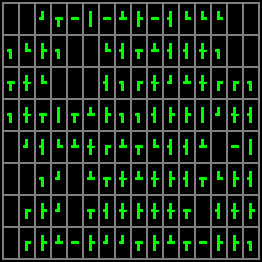
\includegraphics[scale=0.75]{SMT/pipe/shuffled.png}
\caption{Shuffled puzzle}
\end{figure}

\dots and solved:

\begin{figure}[H]
\label{fig:pipe_solved}
\centering
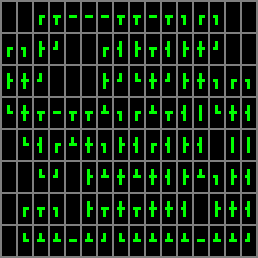
\includegraphics[scale=0.75]{SMT/pipe/solved.png}
\caption{Solved puzzle}
\end{figure}

Let's try to find a way to solve it.

\subsubsection{Generation}

First, we need to generate it.
Here is my quick idea on it.
Take 8*16 array of cells.
Each cell may contain some type of block.
There are joints between cells:

\pgfmathsetmacro\Width{16}
\pgfmathsetmacro\Height{8}
%\pgfmathsetmacro\Width{10}
%\pgfmathsetmacro\Height{5}
\pgfmathtruncatemacro\WidthMinusI{\Width - 1}
\pgfmathtruncatemacro\WidthMinusII{\Width - 2}
\pgfmathtruncatemacro\HeightMinusI{\Height - 1}
\pgfmathtruncatemacro\HeightMinusII{\Height - 2}
\pgfmathtruncatemacro\HeightPlusII{\Height + 2}
\pgfmathsetmacro\HeightPlusIi{\Height + 1.5}

% see also: http://www.texample.net/tikz/examples/euclid-algorithm/
\begin{center}
\begin{tikzpicture}[set style={{help lines}+=[dashed]},scale=0.7]

	\draw[style=help lines] (0,0) grid +(\Width,\Height);

	\foreach \c in {0,...,\WidthMinusI}
	{
		\foreach \r in {0,...,\HeightMinusII}
			\draw   [red,very thick,-] (\c+0.5,\r+0.75) -- (\c+0.5,\r+1.25);
		%\node[rotate=90] at (\c+0.5,\HeightPlusII) {\Large vjoints[\dots, \c] \normalsize};
		\node[rotate=90] at (\c+0.5,\HeightPlusII) {vjoints[\dots, \c]};
	}

	\foreach \r in {0,...,\HeightMinusI}
	{
		\foreach \c in {0,...,\WidthMinusII}
			\draw   [blue,very thick,-] (\c+0.75,\r+0.5) -- (\c+1.25,\r+0.5);
		\pgfmathtruncatemacro\hjointslabel{\HeightMinusI - \r}
		%\node at (-1.5,\r+0.5) {\large hjoints[\hjointslabel, \dots] \normalsize};
		\node at (-1.5,\r+0.5) {hjoints[\hjointslabel, \dots]};
	}

\end{tikzpicture}
\end{center}



Blue lines are horizontal joints, red lines are vertical joints.
We just set each joint to 0/false (absent) or 1/true (present), randomly.

Once set, it's now easy to find type for each cell.
There are:

\newcommand{\HeaderColor}{\cellcolor{blue!25}}
\begin{center}
\begin{longtable}{ | l | l | l | l | }
\hline
\HeaderColor joints & \HeaderColor our internal name & \HeaderColor angle & \HeaderColor symbol \\
\hline
0	&type 0		&	0$^{\circ}$	& (space)	\\
2	&type 2a	&	0$^{\circ}$	& \pmboxdrawuni{2503} \\ % ┃
2	&type 2a	&	90$^{\circ}$	& \pmboxdrawuni{2501} \\ % ━
2	&type 2b	&	0$^{\circ}$	& \pmboxdrawuni{250F} \\ % ┏
2	&type 2b	&	90$^{\circ}$	& \pmboxdrawuni{2513} \\ % ┓
2	&type 2b	&	180$^{\circ}$	& \pmboxdrawuni{251B} \\ % ┛
2	&type 2b	&	270$^{\circ}$	& \pmboxdrawuni{2517} \\ % ┗
3	&type 3		&	0$^{\circ}$	& \pmboxdrawuni{2523} \\ % ┣
3 	&type 3		&	90$^{\circ}$	& \pmboxdrawuni{2533} \\ % ┳
3	&type 3		&	180$^{\circ}$	& \pmboxdrawuni{252B} \\ % ┫
3	&type 3		&	270$^{\circ}$	& \pmboxdrawuni{253B} \\ % ┻
4	&type 4		&	0$^{\circ}$	& \pmboxdrawuni{254B} \\ % ╋
\hline
\end{longtable}
\end{center}

\textit{Dangling} joints can be preset at a first stage (i.e., cell with only one joint), but they are removed recursively,
these cells are transforming into empty cells.
Hence, at the end, all cells has at least two joints, and the whole plumbing system has no connections with outer
world---I hope this would make things clearer.

The C source code of generator is here: \url{https://github.com/dennis714/SAT_SMT_article/tree/master/SMT/pipe/generator}.
All horizontal joints are stored in the global array \textit{hjoints[]} and vertical in \textit{vjoints[]}.

The C program generates ANSI-colored output like it has been showed above (\ref{fig:pipe_shuffled}, \ref{fig:pipe_solved}) plus
an array of types, with no angle information about each cell:

\begin{lstlisting}[label=init_cells]
[
["0", "0", "2b", "3", "2a", "2a", "2a", "3", "3", "2a", "3", "2b", "2b", "2b", "0", "0"],
["2b", "2b", "3", "2b", "0", "0", "2b", "3", "3", "3", "3", "3", "4", "2b", "0", "0"],
["3", "4", "2b", "0", "0", "0", "3", "2b", "2b", "4", "2b", "3", "4", "2b", "2b", "2b"],
["2b", "4", "3", "2a", "3", "3", "3", "2b", "2b", "3", "3", "3", "2a", "2b", "4", "3"],
["0", "2b", "3", "2b", "3", "4", "2b", "3", "3", "2b", "3", "3", "3", "0", "2a", "2a"],
["0", "0", "2b", "2b", "0", "3", "3", "4", "3", "4", "3", "3", "3", "2b", "3", "3"],
["0", "2b", "3", "2b", "0", "3", "3", "4", "3", "4", "4", "3", "0", "3", "4", "3"],
["0", "2b", "3", "3", "2a", "3", "2b", "2b", "3", "3", "3", "3", "2a", "3", "3", "2b"],
]
\end{lstlisting}

\subsubsection{Solving}

First of all, we would think about 8*16 array of cells, where each has four bits:
``T'' (top),
``B'' (bottom),
``L'' (left),
``R'' (right).
Each bit represents half of joint.

% see also: http://www.texample.net/tikz/examples/euclid-algorithm/
\begin{center}
\begin{tikzpicture}[set style={{help lines}+=[dashed]},scale=0.7]

	\draw[style=help lines] (0,0) grid +(\Width,\Height);
	
	\foreach \c in {0,...,\WidthMinusI}
		%\node[rotate=90] at (\c+0.5,\HeightPlusIi) {\Large [\dots, \c] \normalsize};
		\node[rotate=90] at (\c+0.5,\HeightPlusIi) {[\dots, \c]};
	
	\foreach \r in {0,...,\HeightMinusI}
	{
		\pgfmathtruncatemacro\hlabel{\HeightMinusI - \r}
		%\node at (-1.5,\r+0.5) {\large [\hlabel, \dots] \normalsize};
		\node at (-1.5,\r+0.5) {[\hlabel, \dots]};
	
		\pgfmathsetmacro\Shift{0.325}
		\foreach \c in {0,...,\WidthMinusI}
		{
			\node at (\c+0.5,\r+0.5 + \Shift) {\footnotesize T \normalsize};
			\node at (\c+0.5,\r+0.5 - \Shift) {\footnotesize B \normalsize};
			\node at (\c+0.5 - \Shift,\r+0.5) {\footnotesize L \normalsize};
			\node at (\c+0.5 + \Shift,\r+0.5) {\footnotesize R \normalsize};
		}
	}

\end{tikzpicture}
\end{center}


Now we define arrays of each of four half-joints + angle information:

\begin{lstlisting}
HEIGHT=8
WIDTH=16

# if T/B/R/L is Bool instead of Int, Z3 solver will work faster
T=[[Bool('cell_%d_%d_top' % (r, c)) for c in range(WIDTH)] for r in range(HEIGHT)]
B=[[Bool('cell_%d_%d_bottom' % (r, c)) for c in range(WIDTH)] for r in range(HEIGHT)]
R=[[Bool('cell_%d_%d_right' % (r, c)) for c in range(WIDTH)] for r in range(HEIGHT)]
L=[[Bool('cell_%d_%d_left' % (r, c)) for c in range(WIDTH)] for r in range(HEIGHT)]
A=[[Int('cell_%d_%d_angle' % (r, c)) for c in range(WIDTH)] for r in range(HEIGHT)]
\end{lstlisting}

We know that if each of half-joints is present, corresponding half-joint must be also present, and vice versa.
We define this using these constraints:

\begin{lstlisting}
# shorthand variables for True and False:
t=True
f=False

# "top" of each cell must be equal to "bottom" of the cell above
# "bottom" of each cell must be equal to "top" of the cell below
# "left" of each cell must be equal to "right" of the cell at left
# "right" of each cell must be equal to "left" of the cell at right
for r in range(HEIGHT):
    for c in range(WIDTH):
        if r!=0:
            s.add(T[r][c]==B[r-1][c])
        if r!=HEIGHT-1:
            s.add(B[r][c]==T[r+1][c])
        if c!=0:
            s.add(L[r][c]==R[r][c-1])
        if c!=WIDTH-1:
            s.add(R[r][c]==L[r][c+1])

# "left" of each cell of first column shouldn't have any connection
# so is "right" of each cell of the last column
for r in range(HEIGHT):
    s.add(L[r][0]==f)
    s.add(R[r][WIDTH-1]==f)

# "top" of each cell of the first row shouldn't have any connection
# so is "bottom" of each cell of the last row
for c in range(WIDTH):
    s.add(T[0][c]==f)
    s.add(B[HEIGHT-1][c]==f)
\end{lstlisting}

Now we'll enumerate all cells in the initial array (\ref{init_cells}).
First two cells are empty there. And the third one has type ``2b''.
This is ``\pmboxdrawuni{250F}'' % ┏
and it can be oriented in 4 possible ways.
And if it has angle 0$^{\circ}$, bottom and right half-joints are present, others are absent.
If it has angle 90$^{\circ}$, it looks like 
``\pmboxdrawuni{2513}'', % ┓
and bottom and left half-joints are present, others are absent.

In plain English: ``if cell of this type has angle 0$^{\circ}$, these half-joints must be present \textbf{OR}
if it has angle 90$^{\circ}$, these half-joints must be present, \textbf{OR}, etc, etc.''

Likewise, we define all these rules for all types and all possible angles:

\begin{lstlisting}
for r in range(HEIGHT):
    for c in range(WIDTH):
        ty=cells_type[r][c]

        if ty=="0":
            s.add(A[r][c]==f)
            s.add(T[r][c]==f, B[r][c]==f, L[r][c]==f, R[r][c]==f)

        if ty=="2a":
            s.add(Or(And(A[r][c]==0, L[r][c]==f, R[r][c]==f, T[r][c]==t, B[r][c]==t),   # §\pmboxdrawuni{2503}§
                    And(A[r][c]==90, L[r][c]==t, R[r][c]==t, T[r][c]==f, B[r][c]==f)))  # §\pmboxdrawuni{2501}§

        if ty=="2b":
            s.add(Or(And(A[r][c]==0, L[r][c]==f, R[r][c]==t, T[r][c]==f, B[r][c]==t),   # §\pmboxdrawuni{250F}§
                    And(A[r][c]==90, L[r][c]==t, R[r][c]==f, T[r][c]==f, B[r][c]==t),   # §\pmboxdrawuni{2513}§
                    And(A[r][c]==180, L[r][c]==t, R[r][c]==f, T[r][c]==t, B[r][c]==f),  # §\pmboxdrawuni{251B}§
                    And(A[r][c]==270, L[r][c]==f, R[r][c]==t, T[r][c]==t, B[r][c]==f))) # §\pmboxdrawuni{2517}§
	
        if ty=="3":
            s.add(Or(And(A[r][c]==0, L[r][c]==f, R[r][c]==t, T[r][c]==t, B[r][c]==t),   # §\pmboxdrawuni{2523}§
                    And(A[r][c]==90, L[r][c]==t, R[r][c]==t, T[r][c]==f, B[r][c]==t),   # §\pmboxdrawuni{2533}§
                    And(A[r][c]==180, L[r][c]==t, R[r][c]==f, T[r][c]==t, B[r][c]==t),  # §\pmboxdrawuni{252B}§
                    And(A[r][c]==270, L[r][c]==t, R[r][c]==t, T[r][c]==t, B[r][c]==f))) # §\pmboxdrawuni{253B}§

        if ty=="4":
            s.add(A[r][c]==0)
            s.add(T[r][c]==t, B[r][c]==t, L[r][c]==t, R[r][c]==t) # §\pmboxdrawuni{254B}§
\end{lstlisting}

Full source code is here: \url{https://github.com/dennis714/SAT_SMT_article/blob/master/SMT/pipe/solver/solve_pipe_puzzle1.py}.

It produces this result (prints angle for each cell and (pseudo)graphical representation):

\begin{figure}[H]
\centering
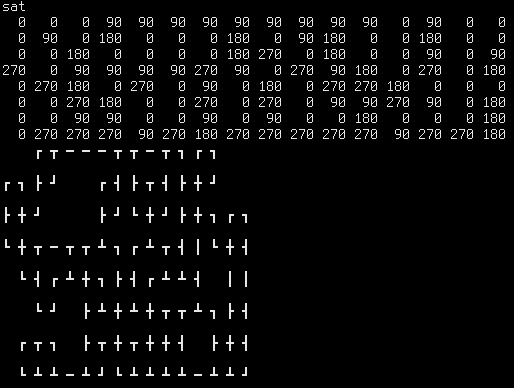
\includegraphics[scale=0.75]{SMT/pipe/solver/solver.png}
\caption{Solver script output}
\end{figure}

It worked $\approx 4$ seconds on my old and slow Intel Atom N455 1.66GHz.
Is it fast? I don't know, but again, what is really cool, we do not know about any mathematical background
of all this, we just defined cells, (half-)joints and defined relations between them.

Now the next question is, how many solutions are possible?
Using method described earlier (\ref{SMTEnumerate}), I've altered solver script
\footnote{\url{https://github.com/dennis714/SAT_SMT_article/blob/master/SMT/pipe/solver/solve_pipe_puzzle2.py}} and solver
said two solutions are possible.

Let's compare these two solutions using gvimdiff:

\begin{figure}[H]
\centering
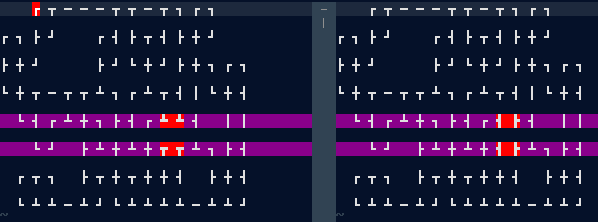
\includegraphics[scale=0.75]{SMT/pipe/solver/diff.png}
\caption{gvimdiff output (pardon my red cursor at left pane at left-bottom corner)}
\end{figure}

4 cells in the middle can be orientated differently.
Perhaps, other puzzles may produce different results.

P.S.
\textit{Half-joint} is defined as boolean type.
But in fact, the first version of the solver has been written using integer type for half-joints,
and 0 was used for False and 1 for True.
I did it so because I wanted to make source code tidier and narrower without using long words like ``False'' and ``True''.
And it worked, but slower. Perhaps, Z3 handles boolean data types faster? Better?
Anyway, I writing this to note that integer type can also be used instead of boolean, if needed.


\subsection{Cracking Minesweeper with Z3 SMT solver}
\label{minesweeper_SMT}

For those who are not very good at playing Minesweeper (like me), it's possible to predict bombs' placement without touching debugger.

Here is a clicked somewhere and I see revealed empty cells and cells with known number of ``neighbours'':

\begin{figure}[H]
\centering
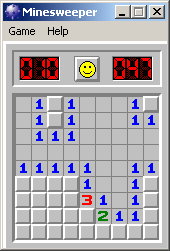
\includegraphics[scale=0.75]{SMT/minesweeper/1.png}
\end{figure}

What we have here, actually? Hidden cells, empty cells (where bombs are not present), and empty cells with numbers, which shows how many bombs are placed nearby.

\subsubsection{The method}

Here is what we can do: we will try to place a bomb to all possible hidden cells and ask Z3 SMT solver, if it can disprove the very fact that the bomb can be placed there.

Take a look at this fragment. "?" mark is for hidden cell, "." is for empty cell, number is a number of neighbours.

\begin{center}
\begin{tabular}{ | c | c | c | c | }
\hline
 & C1 & C2 & C3 \\
\hline
R1 & ? & ? & ? \\
\hline
R2 & ? & 3 & . \\
\hline
R3 & ? & 1 & . \\
\hline
\end{tabular}
\end{center}

So there are 5 hidden cells.
We will check each hidden cell by placing a bomb there.
Let's first pick top/left cell:

\begin{center}
\begin{tabular}{ | c | c | c | c | }
\hline
 & C1 & C2 & C3 \\
\hline
R1 & * & ? & ? \\
\hline
R2 & ? & 3 & . \\
\hline
R3 & ? & 1 & . \\
\hline
\end{tabular}
\end{center}

Then we will try to solve the following system of equations (\textit{RrCc} is cell of row $r$ and column $c$):

\begin{itemize}
\item R1C2+R2C1+R2C2=1                               (because we placed bomb at R1C1)	
\item R2C1+R2C2+R3C1=1                               (because we have "1" at R3C2)	
\item R1C1+R1C2+R1C3+R2C1+R2C2+R2C3+R3C1+R3C2+R3C3=3 (because we have "3" at R2C2)	
\item R1C2+R1C3+R2C2+R2C3+R3C2+R3C3=0                (because we have "." at R2C3)	
\item R2C2+R2C3+R3C2+R3C3=0                          (because we have "." at R3C3)
\end{itemize}

As it turns out, this system of equations is satisfiable, so there could be a bomb at this cell.
But this information is not interesting to us, since we want to find cells we can freely click on.
And we will try another one.
And if the equation will be unsatisfiable, that would imply that a bomb cannot be there and we can click on it.

\subsubsection{The code}

\lstinputlisting{SMT/minesweeper/minesweeper_solver.py}

The code is almost self-explanatory.
We need border for the same reason, why Conway's "Game of Life" implementations also has border (to make calculation
function simpler).
Whenever we know that the cell is free of bomb, we put zero there.
Whenever we know number of neighbours, we add a constraint, again, just like in "Game of Life": number of neighbours must be equal to the number we have seen in the Minesweeper.
Then we place bomb somewhere and check.

Let's run:

\begin{lstlisting}
row=1 col=3, unsat!
row=6 col=2, unsat!
row=6 col=3, unsat!
row=7 col=4, unsat!
row=7 col=9, unsat!
row=8 col=9, unsat!
\end{lstlisting}

These are cells where I can click safely, so I did:

\begin{figure}[H]
\centering
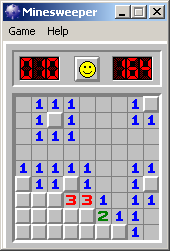
\includegraphics[scale=0.75]{SMT/minesweeper/2.png}
\end{figure}

Now we have more information, so we update input:

\begin{lstlisting}
known=[
"01110001?",
"01?100011",
"011100000",
"000000000",
"111110011",
"?11?1001?",
"???331011",
"?????2110",
"???????10"]
\end{lstlisting}

I run it again:

\begin{lstlisting}
row=7 col=1, unsat!
row=7 col=2, unsat!
row=7 col=3, unsat!
row=8 col=3, unsat!
row=9 col=5, unsat!
row=9 col=6, unsat!
\end{lstlisting}

I click on these cells again:

\begin{figure}[H]
\centering
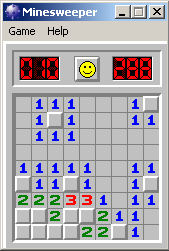
\includegraphics[scale=0.75]{SMT/minesweeper/3.png}
\end{figure}

I update it again:

\begin{lstlisting}
known=[
"01110001?",
"01?100011",
"011100000",
"000000000",
"111110011",
"?11?1001?",
"222331011",
"??2??2110",
"????22?10"]
\end{lstlisting}

\begin{lstlisting}
row=8 col=2, unsat!
row=9 col=4, unsat!
\end{lstlisting}

\begin{figure}[H]
\centering
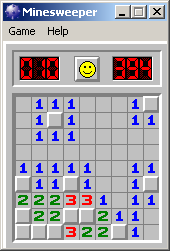
\includegraphics[scale=0.75]{SMT/minesweeper/4.png}
\end{figure}

This is last update:

\begin{lstlisting}
known=[
"01110001?",
"01?100011",
"011100000",
"000000000",
"111110011",
"?11?1001?",
"222331011",
"?22??2110",
"???322?10"]
\end{lstlisting}

\dots last result:

\begin{lstlisting}
row=9 col=1, unsat!
row=9 col=2, unsat!
\end{lstlisting}

Voila!

\begin{figure}[H]
\centering
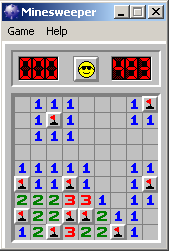
\includegraphics[scale=0.75]{SMT/minesweeper/5.png}
\end{figure}

The source code: \url{https://github.com/dennis714/SAT_SMT_article/blob/master/SMT/minesweeper/minesweeper_solver.py}.

Some discussion on HN: \url{https://news.ycombinator.com/item?id=13797375}.

See also: cracking Minesweeper using SAT solver: \ref{minesweeper_SAT}.


\subsection{Recalculating micro-spreadsheet using Z3Py}

There is a nice exercise\footnote{Blog post in Russian: \url{http://thesz.livejournal.com/280784.html}}:
write a program to recalculate micro-spreadsheet, like this one:

\lstinputlisting{SMT/spreadsheet/test1}

As it turns out, though overkill, this can be solved using Z3 with little effort:

\lstinputlisting{SMT/spreadsheet/1.py}

( \url{https://github.com/dennis714/yurichev.com/blob/master/blog/spreadsheet/1.py} )

All we do is just creating pack of variables for each cell, named A0, B1, etc, of integer type.
All of them are stored in \textit{cells[]} dictionary.
Key is a string.
Then we parse all the strings from cells, and add to list of constraints \textit{A0=123}
(in case of number in cell) or \textit{A0=B1+C2} (in case of expression in cell).
There is a slight preparation: string like \textit{A0+B2} becomes \textit{cells["A0"]+cells["B2"]}.

Then the string is evaluated using Python \textit{eval()} method,
which is highly dangerous
\footnote{\url{http://stackoverflow.com/questions/1832940/is-using-eval-in-python-a-bad-practice}}:
imagine if end-user could add a string to cell other than expression?
Nevertheless, it serves our purposes well, because this is a simplest way to pass a string with expression into Z3.

Z3 do the job with little effort:

\begin{lstlisting}
 % python 1.py test1
sat
1       0       135     82041
123     10      12      11
667     11      1342    83383
\end{lstlisting}

\subsubsection{Unsat core}

Now the problem: what if there is circular dependency? Like:

\lstinputlisting{SMT/spreadsheet/test_circular}

Two first cells of the last row (C0 and C1) are linked to each other.
Our program will just tells ``unsat'', meaning, it couldn't satisfy all constraints together.
We can't use this as error message reported to end-user, because it's highly unfriendly.

However, we can fetch \textit{unsat core}, i.e., list of variables which Z3 finds conflicting.

\begin{lstlisting}
...
s=Solver()
s.set(unsat_core=True)
...
        # add constraint:
        s.assert_and_track(e, coord_to_name(cur_R, cur_C))
...
if result=="sat":
...
else:
    print s.unsat_core()
\end{lstlisting}

( \url{https://github.com/dennis714/yurichev.com/blob/master/blog/spreadsheet/2.py} )

We should explicitly turn on unsat core support and use \textit{assert\_and\_track()} instead of \textit{add()} method,
because this feature slows down the whole process, and is turned off by default.
That works:

\begin{lstlisting}
 % python 2.py test_circular
unsat
[C0, C1]
\end{lstlisting}

Perhaps, these variables could be removed from the 2D array, marked as \textit{unresolved}
and the whole spreadsheet could be recalculated again.

\subsubsection{Stress test}

How to generate large random spreadsheet?
What we can do.
First, create random \ac{DAG}, like this one:

\begin{figure}[H]
\centering
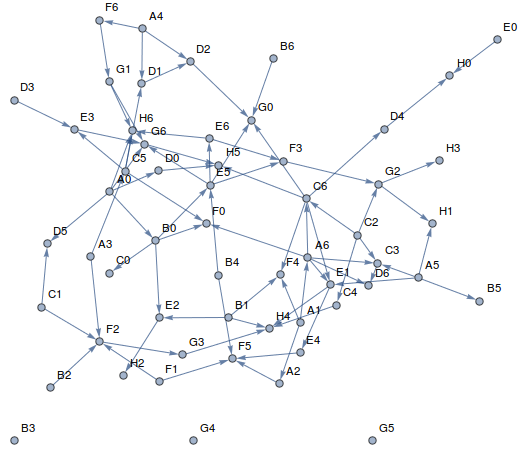
\includegraphics[width=\textwidth]{SMT/spreadsheet/1.png}
\caption{Random DAG}
\end{figure}

Arrows will represent information flow.
So a vertex (node) which has no incoming arrows to it (indegree=0), can be set to a random number.
Then we use topological sort to find dependencies between vertices.
Then we assign spreadsheet cell names to each vertex.
Then we generate random expression with random operations/numbers/cells to each cell,
with the use of information from topological sorted graph.

\begin{lstlisting}
(* Utility functions *)
In[1]:= findSublistBeforeElementByValue[lst_,element_]:=lst[[ 1;;Position[lst, element][[1]][[1]]-1]]

(* Input in 1..∞ range. 1->A0, 2->A1, etc *)
In[2]:= vertexToName[x_,width_]:=StringJoin[FromCharacterCode[ToCharacterCode["A"][[1]]+Floor[(x-1)/width]],ToString[Mod[(x-1),width]]]

In[3]:= randomNumberAsString[]:=ToString[RandomInteger[{1,1000}]]

In[4]:= interleaveListWithRandomNumbersAsStrings[lst_]:=Riffle[lst,Table[randomNumberAsString[],Length[lst]-1]]

(* We omit division operation because micro-spreadsheet evaluator can't handle division by zero *)
In[5]:= interleaveListWithRandomOperationsAsStrings[lst_]:=Riffle[lst,Table[RandomChoice[{"+","-","*"}],Length[lst]-1]]

In[6]:= randomNonNumberExpression[g_,vertex_]:=StringJoin[interleaveListWithRandomOperationsAsStrings[interleaveListWithRandomNumbersAsStrings[Map[vertexToName[#,WIDTH]&,pickRandomNonDependentVertices[g,vertex]]]]]

In[7]:= pickRandomNonDependentVertices[g_,vertex_]:=DeleteDuplicates[RandomChoice[findSublistBeforeElementByValue[TopologicalSort[g],vertex],RandomInteger[{1,5}]]]

In[8]:= assignNumberOrExpr[g_,vertex_]:=If[VertexInDegree[g,vertex]==0,randomNumberAsString[],randomNonNumberExpression[g,vertex]]

(* Main part *) 
(* Create random graph *)
In[21]:= WIDTH=7;HEIGHT=8;TOTAL=WIDTH*HEIGHT
Out[21]= 56

In[24]:= g=DirectedGraph[RandomGraph[BernoulliGraphDistribution[TOTAL,0.05]],"Acyclic"];

...

(* Generate random expressions and numbers *)
In[26]:= expressions=Map[assignNumberOrExpr[g,#]&,VertexList[g]];

(* Make 2D table of it *)
In[27]:= t=Partition[expressions,WIDTH];

(* Export as tab-separated values *)
In[28]:= Export["/home/dennis/1.txt",t,"TSV"]
Out[28]= /home/dennis/1.txt

In[29]:= Grid[t,Frame->All,Alignment->Left]
\end{lstlisting}

Here is an output from \textit{Grid[]}:

% FIXME: size!
\tiny
\begin{center}
\begin{tabular}{ | l | l | l | l | l | l | l |}
\hline
846 & 499 & A3*913-H4 & 808 & 278 & 303 & D1+579+B6 \\
\hline
B4*860+D2 & 999 & 59 & 442 & 425 & A5*163+B2+127*C2*927*D3*213+C1 & 583 \\
\hline
G6*379-C3-436-C4-289+H6 & 972 & 804 & D2 & G5+108-F1*413-D3 & B5 & G4*981*D2 \\
\hline
F2 & E0 & B6-731-D3+791+B4*92+C1 & 551 & F4*922*C2+760*A6-992+B4-184-A4 & B1-624-E3 & F4+182+A4*940-E1+76*C1 \\
\hline
519 & G1*402+D1*107*G3-458*A1 & D3 & B4 & B3*811-D3*345+E0 & B5 & H5 \\
\hline
F5-531+B5-222*E4 & 9 & B5+106*B6+600-B1 & E3 & A5+866*F6+695-A3*226+C6 & F4*102*E4*998-H0 & B1-616-G5+812-A5 \\
\hline
C3-956*A5 & G4*408-D3*290*B6-899*G5+400+F1 & B2-701+H6 & A3+782*A5+46-B3-731+C1 & 42 & 287 & H0 \\
\hline
B4-792*H4*407+F6-425-E1 & D2 & D3 & F2-327*G4*35*E1 & E1+376*A6-606*F6*554+C5 & E3 & F6*484+C1-114-H4-638-A3 \\
\hline
\end{tabular}
\end{center}
\normalsize



Using this script, I can generate random spreadsheet of $26 \cdot 500=13000$ cells,
which seems to be processed in couple of seconds.

\subsubsection{The files}

The files, including Mathematica notebook: \url{https://github.com/dennis714/yurichev.com/tree/master/blog/spreadsheet}.


\subsection{Discrete tomography}

How computed tomography (CT scan) actually works?
A human body is bombarded by X-rays in various angles by X-ray tube in rotating torus.
X-ray detectors are also located in torus, and all the information is recorded.

Here is we can simulate simple tomograph.
An ``i'' character is rotating and will be ``enlighten'' at 4 angles.
Let's imagine, character is bombarded by X-ray tube at left.
All asterisks in each row is then summed and sum is "received" by X-ray detector at the right.

\begin{lstlisting}
WIDTH= 11 HEIGHT= 11
angle=(π/4)*0
    **      2
    **      2
            0
   ***      3
    **      2
    **      2
    **      2
    **      2
    **      2
   ****     4
            0
[2, 2, 0, 3, 2, 2, 2, 2, 2, 4, 0] ,
angle=(π/4)*1
            0
            0
  *         1
 **         2
    *       1
    **      2
     **     2
     ****   4
       *    1
      *     1
            0
[0, 0, 1, 2, 1, 2, 2, 4, 1, 1, 0] ,
angle=(π/4)*2
            0
            0
            0
            0
         *  1
** *******  9
** *******  9
   *     *  2
            0
            0
            0
[0, 0, 0, 0, 1, 9, 9, 2, 0, 0, 0] ,
angle=(π/4)*3
            0
            0
       *    1
       **   2
      ** *  3
     ***    3
    **      2
            0
  **        2
   *        1
            0
[0, 0, 1, 2, 3, 3, 2, 0, 2, 1, 0] ,
\end{lstlisting}

( The source code: \url{https://github.com/dennis714/SAT_SMT_article/blob/master/SMT/tomo/gen.py} )

All we got from our toy-level tomograph is 4 vectors, these are sums of all asterisks in rows for 4 angles:

\begin{lstlisting}
[2, 2, 0, 3, 2, 2, 2, 2, 2, 4, 0] ,
[0, 0, 1, 2, 1, 2, 2, 4, 1, 1, 0] ,
[0, 0, 0, 0, 1, 9, 9, 2, 0, 0, 0] ,
[0, 0, 1, 2, 3, 3, 2, 0, 2, 1, 0] ,
\end{lstlisting}

How do we recover initial image?
We are going to represent 11*11 matrix, where sum of each row must be equal to some value we already know.
Then we rotate matrix, and do this again.

For the first matrix, the system of equations looks like that (we put there a values from the first vector):

\begin{lstlisting}
C1,1 + C1,2 + C1,3 + ... + C1,11 =      2
C2,1 + C2,2 + C2,3 + ... + C2,11 =      2

...

C10,1 + C10,2 + C10,3 + ... + C10,11 =  4
C11,1 + C11,2 + C11,3 + ... + C11,11 =  0
\end{lstlisting}

We also build similar systems of equations for each angle.

The ``rotate'' function has been taken from the generation program, because, due to Python's dynamic typization nature,
it's not important for the function to what operate on:
strings, characters, or Z3 variable instances, so it works very well for all of them.

\begin{lstlisting}
#-*- coding: utf-8 -*-

import math, sys
from z3 import *

# https://en.wikipedia.org/wiki/Rotation_matrix
def rotate(pic, angle):
    WIDTH=len(pic[0])
    HEIGHT=len(pic)
    #print WIDTH, HEIGHT
    assert WIDTH==HEIGHT
    ofs=WIDTH/2

    out = [[0 for x in range(WIDTH)] for y in range(HEIGHT)]

    for x in range(-ofs,ofs):
        for y in range(-ofs,ofs):
            newX = int(round(math.cos(angle)*x - math.sin(angle)*y,3))+ofs
            newY = int(round(math.sin(angle)*x + math.cos(angle)*y,3))+ofs
            # clip at boundaries, hence min(..., HEIGHT-1)
            out[min(newX,HEIGHT-1)][min(newY,WIDTH-1)]=pic[x+ofs][y+ofs]
    return out

vectors=[
[2, 2, 0, 3, 2, 2, 2, 2, 2, 4, 0] ,
[0, 0, 1, 2, 1, 2, 2, 4, 1, 1, 0] ,
[0, 0, 0, 0, 1, 9, 9, 2, 0, 0, 0] ,
[0, 0, 1, 2, 3, 3, 2, 0, 2, 1, 0]]

WIDTH = HEIGHT = len(vectors[0])

s=Solver()
cells=[[Int('cell_r=%d_c=%d' % (r,c)) for c in range(WIDTH)] for r in range(HEIGHT)]

# monochrome picture, only 0's or 1's:
for c in range(WIDTH):
    for r in range(HEIGHT):
        s.add(Or(cells[r][c]==0, cells[r][c]==1))

def all_zeroes_in_vector(vec):
    for v in vec:
        if v!=0:
            return False
    return True

ANGLES=len(vectors)
for a in range(ANGLES):
    angle=a*(math.pi/ANGLES)
    rows=rotate(cells, angle)
    r=0
    for row in rows:
        # skip empty rows:
        if all_zeroes_in_vector(row)==False:
            # sum of row must be equal to the corresponding element of vector:
            s.add(Sum(*row)==vectors[a][r])
        r=r+1

print s.check()
m=s.model()
for r in range(HEIGHT):
    for c in range(WIDTH):
        if str(m[cells[r][c]])=="1":
            sys.stdout.write("*")
        else:
            sys.stdout.write(" ")
    print ""
\end{lstlisting}

( The source code: \url{https://github.com/dennis714/SAT_SMT_article/blob/master/SMT/tomo/solve.py} )

That works:

\begin{lstlisting}
% python solve.py
sat
    **
    **

   ***
    **
    **
    **
    **
    **
   ****
\end{lstlisting}

In other words, all SMT-solver does here is solving a system of equations.

So, 4 angles are enough.
What if we could use only 3 angles?

\begin{lstlisting}
WIDTH= 11 HEIGHT= 11
angle=(π/3)*0
    **      2
    **      2
            0
   ***      3
    **      2
    **      2
    **      2
    **      2
    **      2
   ****     4
            0
[2, 2, 0, 3, 2, 2, 2, 2, 2, 4, 0] ,
angle=(π/3)*1
            0
            0
            0
 **         2
 **         2
   ***      3
     ****   4
       **   2
       *    1
            0
            0
[0, 0, 0, 2, 2, 3, 4, 2, 1, 0, 0] ,
angle=(π/3)*2
            0
            0
            0
       **   2
       **   2
     *****  5
    **      2
 **         2
  *         1
            0
            0
[0, 0, 0, 2, 2, 5, 2, 2, 1, 0, 0] ,
\end{lstlisting}

No, it's not enough:

\begin{lstlisting}
% time python solve3.py
sat
 *  *
    **

     * **
   **
   *  *
    **
     *   *
*   *
   ****
\end{lstlisting}

However, the result is correct, but only 3 vectors allows too many possible ``initial images'',
and Z3 SMT-solver finds first.

Further reading:
\url{https://en.wikipedia.org/wiki/Discrete_tomography},
\url{https://en.wikipedia.org/wiki/2-satisfiability#Discrete_tomography}.


\subsection{Simplifying long and messy expressions using Mathematica and Z3}

\dots which can be results of Hex-Rays and/or manual rewriting.

I've added to my RE4B book about Wolfram Mathematica capabilities to minimize expressions
\footnote{\url{https://github.com/dennis714/RE-for-beginners/blob/cd85356051937e87f90967cc272248084808223b/other/hexrays_EN.tex\#L412}, \url{https://beginners.re/}}.

Today I stumbled upon this Hex-Rays output:

\begin{lstlisting}
if ( ( x != 7 || y!=0 ) && (x < 6 || x > 7) )
{
        ...
};
\end{lstlisting}

Both Mathematica and Z3 (using ``simplify'' command) can't make it shorter, but I've got gut feeling,
that there is something redundant.

Let's take a look at the right part of the expression.
If $x$ must be less than 6 \textit{OR} greater than 7, then it can hold any value except 6 \textit{AND} 7, right?
So I can rewrite this manually:

\begin{lstlisting}
if ( ( x != 7 || y!=0 ) && x != 6 && x != 7) )
{
        ...
};
\end{lstlisting}

And this is what Mathematica can simplify:

\begin{lstlisting}
In[]:= BooleanMinimize[(x != 7 || y != 0) && (x != 6 && x != 7)]
Out[]:= x != 6 && x != 7
\end{lstlisting}

$y$ gets reduced.

But am I really right?
And why Mathematica and Z3 didn't simplify this at first place?

I can use Z3 to prove that these expressions are equal to each other:

\begin{lstlisting}
#!/usr/bin/env python

from z3 import *

x=Int('x')
y=Int('y')

s=Solver()

exp1=And(Or(x!=7, y!=0), Or(x<6, x>7))
exp2=And(x!=6, x!=7)

s.add(exp1!=exp2)

print simplify(exp1) # no luck

print s.check()
print s.model()
\end{lstlisting}

Z3 can't find counterexample, so it says ``unsat'', meaning, these expressions are equivalent to each other.
So I've rewritten this expression in my code, tests has been passed, etc.

Yes, using both Mathematica and Z3 is overkill, and this is basic boolean algebra,
but after \textasciitilde{}10 hours of sitting at a computer you can make really dumb mistakes,
and additional proof your piece of code is correct is never unwanted.


\subsection{Solving XKCD 287 using Z3}

\begin{figure}[H]
\centering
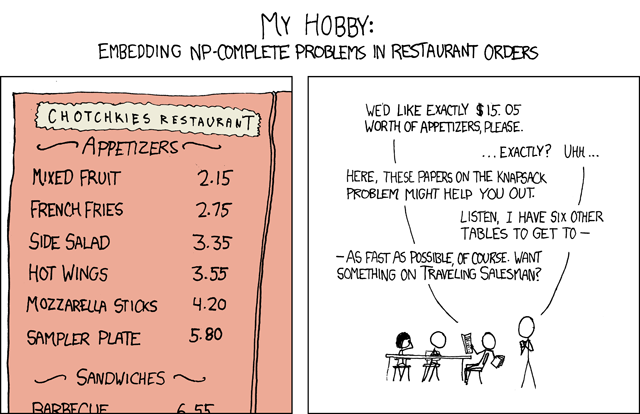
\includegraphics[scale=7]{SMT/xkcd287/np_complete.png}
\caption{xkcd \#287}
\end{figure}

( \url{https://www.xkcd.com/287/} )

The problem is to solve the following equation:
$2.15a + 2.75b + 3.35c + 3.55d + 4.20e + 5.80f == 15.05$,
where a..f are integers.
So this is a linear diophantine equation.

\begin{lstlisting}
#!/usr/bin/python

from z3 import *

a,b,c,d,e,f = Ints('a b c d e f')
s = Solver()
s.add(215*a + 275*b + 335*c + 355*d + 420*e + 580*f == 1505, a>=0, b>=0, c>=0, d>=0, e>=0, f>=0)

results=[]

# enumerate all possible solutions:
while True:
    if s.check() == sat:
        m = s.model()
        print m
        results.append(m)
        block = []
        for d in m:
            c=d()
            block.append(c != m[d])
        s.add(Or(block))
    else:
        print "results total=", len(results)
        break
\end{lstlisting}

( The source code: \url{https://github.com/dennis714/SAT_SMT_article/blob/master/SMT/xkcd287/xkcd287.py} )

There are just 2 solutions:

\begin{lstlisting}
[f = 0, b = 0, a = 7, c = 0, d = 0, e = 0]
[f = 1, b = 0, a = 1, c = 0, d = 2, e = 0]
results total= 2
\end{lstlisting}

Wolfram Mathematica can solve the equation as well:

\begin{lstlisting}
In[]:= FindInstance[2.15 a + 2.75 b + 3.35 c + 3.55 d + 4.20 e + 5.80 f == 15.05 && 
	a >= 0 && b >= 0 && c >= 0 && d >= 0  && e >= 0 && f >= 0, 
	{a, b, c, d, e, f}, Integers, 1000]

Out[]= {{a -> 1, b -> 0, c -> 0, d -> 2, e -> 0, f -> 1},
	{a -> 7, b -> 0, c -> 0, d -> 0, e -> 0, f -> 0}}
\end{lstlisting}

1000 means ``find at most 1000 solutions'', but only 2 are found.
See also: \url{http://reference.wolfram.com/language/ref/FindInstance.html}.\\
\\
Other ways to solve it:
\url{https://stackoverflow.com/questions/141779/solving-the-np-complete-problem-in-xkcd},
\url{http://www.explainxkcd.com/wiki/index.php/287:_NP-Complete}.


\subsection{Making smallest possible test suite using Z3}
\label{set_cover}

I once worked on rewriting large piece of code into pure C, and there were a tests, several thousands.
Testing process was painfully slow, so I thought if the test suite can be minimized somehow.

What we can do is to run each test and get code coverage
(information about which lines of code was executed and which are not).
Then the task is to make such test suite, where coverage is maximum, and number of tests is minimal.

In fact, this is \textit{set cover problem} (also known as \textit{hitting set problem}).
While simpler algorithms exist (see Wikipedia\footnote{\url{https://en.wikipedia.org/wiki/Set_cover_problem}}),
it is also possible to solve with SMT-solver.

First, I took \ac{LZSS} compression/decompression code
\footnote{\url{https://github.com/opensource-apple/kext_tools/blob/master/compression.c}} for the example,
from Apple sources.
Such routines are not easy to test.
Here is my version of it:
\url{https://github.com/dennis714/SAT_SMT_article/blob/master/SMT/set_cover/compression.c}.
I've added random generation of input data to be compressed.
Random generation is dependent of some kind of input seed.
Standard \TT{srand()}/\TT{rand()} are not recommended to be used, but for such simple task as ours, it's OK.
I'll generate\footnote{\url{https://github.com/dennis714/yurichev.com/blob/master/blog/set_cover/gen_gcov_tests.sh}}
1000 tests with 0..999 seeds, that would produce random data to be compressed/decompressed/checked.

After the compression/decompression routine has finished its work,
GNU gcov utility is executed, which produces result like this:

\begin{lstlisting}
...
     3395:  189:        for (i = 1; i < F; i++) {
     3395:  190:            if ((cmp = key[i] - sp->text_buf[p + i]) != 0)
     2565:  191:                break;
        -:  192:        }
     2565:  193:        if (i > sp->match_length) {
     1291:  194:            sp->match_position = p;
     1291:  195:            if ((sp->match_length = i) >= F)
    #####:  196:                break;
        -:  197:        }
     2565:  198:    }
    #####:  199:    sp->parent[r] = sp->parent[p];
    #####:  200:    sp->lchild[r] = sp->lchild[p];
    #####:  201:    sp->rchild[r] = sp->rchild[p];
    #####:  202:    sp->parent[sp->lchild[p]] = r;
    #####:  203:    sp->parent[sp->rchild[p]] = r;
    #####:  204:    if (sp->rchild[sp->parent[p]] == p)
    #####:  205:        sp->rchild[sp->parent[p]] = r;
...
\end{lstlisting}

A leftmost number is an execution count for each line.
\TT{\#\#\#\#\#} means the line of code hasn't been executed at all.
The second column is a line number.

Now the Z3Py script, which will parse all these 1000 gcov results and produce minimal \textit{hitting set}:

\lstinputlisting{SMT/set_cover/set_cover.py}

And what it produces (\textasciitilde{}19s on my old Intel Quad-Core Xeon E3-1220 3.10GHz):

\begin{lstlisting}
% time python set_cover.py
sat
test_7
test_48
test_134
python set_cover.py  18.95s user 0.03s system 99% cpu 18.988 total
\end{lstlisting}

We need just these 3 tests to execute (almost) all lines in the code:
looks impressive, given the fact, that it would be notoriously hard to pick these tests by hand!
The result can be checked easily, again, using gcov utility.

This is sometimes also called MaxSAT/MaxSMT --- the problem is to find solution,
but the solution where some variable/expression is maximal as possible, or minimal as possible.

Also, the code gives incorrect results on Z3 4.4.1, but working correctly on Z3 4.5.0 (so please upgrade).
This is relatively fresh feature in Z3, so probably it was not stable in previous versions?

The files: \url{https://github.com/dennis714/SAT_SMT_article/tree/master/SMT/set_cover}.

Further reading:
\url{https://en.wikipedia.org/wiki/Set_cover_problem},
\url{https://en.wikipedia.org/wiki/Maximum_satisfiability_problem},
\url{https://en.wikipedia.org/wiki/Optimization_problem}.


\subsection{Package manager and Z3}

Here is simplified example.
We have libA, libB, libC and libD, available in various versions (and flavors).
We're going to install programA and programB, which use these libraries.

\lstinputlisting{SMT/dep/dependency.py}

( The source code: \url{https://github.com/dennis714/SAT_SMT_article/blob/master/SMT/dep/dependency.py} )

The output:

\begin{lstlisting}
sat
[libB = 5,
 libD = 999,
 libC = 10,
 programB = 7,
 programA = 1,
 libA = 2]
\end{lstlisting}

999 means that there is no need to install libD, it's not required by other packages.

Change version of ProgramB to v8 and it will says ``unsat'', meaning, there is a conflict:
ProgramA requires libA v2, but ProgramB v8 eventually requires newer libA.

Still, there is a work to do: ``unsat'' message is somewhat useless to end user,
some information about conflicting items should be printed.

Here is my another optimization problem example: \ref{set_cover}.

More about using SAT/SMT solvers in package managers: \url{https://research.swtch.com/version-sat},
\url{https://cseweb.ucsd.edu/~lerner/papers/opium.pdf}.

Now in the opposite direction: forcing aptitude package manager to solve Sudoku: \\
\url{http://web.archive.org/web/20160326062818/http://algebraicthunk.net/~dburrows/blog/entry/package-management-sudoku/}.

Some readers may ask, how to order libraries/programs/packages to be installed?
This is simpler problem, which is often solved by topological sorting.
The algorithm reorders graph in such a way so that vertices not depended on anything will be on the top of queue.
Next, there will be vertices dependend on vertices from the previous layer.
And so on.

\textit{make} UNIX utility does this while constructing order of items to be processed.
Even more: older \textit{make} utilities offloaded the job to the external utility (\textit{tsort}).
Some older UNIX has it, at least some versions of NetBSD
\footnote{\url{http://netbsd.gw.com/cgi-bin/man-cgi/man?tsort+1+NetBSD-current}}.


\subsection{Cracking simple XOR cipher with Z3}

Here is a problem: a text encrypted with simple XOR cipher.
Trying all possible keys is not an option.

Relationships between plain text, cipher text and key can be described using simple system of equations.
But we can do more: we can ask Z3 to find such a key (array of bytes), so the plain text will have as many lowercase
letters (a...z) as possible, but a solution will still satisfy all conditions.

\lstinputlisting{SMT/XOR/1.py}

( The source code: \url{https://github.com/dennis714/SAT_SMT_article/blob/master/SMT/XOR/1.py} )

Let's try it on a small 350-bytes file\footnote{\url{https://github.com/dennis714/SAT_SMT_article/blob/master/SMT/XOR/cipher1.txt}}:

\begin{lstlisting}
% python 1.py cipher1.txt
len= 1
len= 2
len= 3
len= 4
len= 5

...

len= 16
len= 17
key=
00000000: 90 A0 21 52 48 84 FB FF  86 83 CF 50 46 12 7A F9  ..!RH......PF.z.
00000010: 36                                                6
plain=
00000000: 4D 72 2E 22 54 63 65 72  6F 6F 63 6D 27 48 6F 6C  Mr."Tceroocm'Hol
00000010: 6A 65 73 2C 22 70 63 6F  20 74 61 73 26 72 73 75  jes,"pco tas&rsu
00000020: 61 6B 6C 79 20 74 62 79  79 20 6F 61 74 63 27 69  akly tbyy oatc'i
00000030: 6E 20 73 68 65 20 6F 68  79 6E 69 6D 67 73 2A 27  n she ohynimgs*'
00000040: 73 61 76 62 0D 0A 75 72  68 65 20 74 6B 6F 73 63  savb..urhe tkosc
00000050: 27 6E 6F 74 27 69 6E 66  70 62 7A 75 65 6D 74 20  'not'infpbzuemt
00000060: 69 64 63 61 73 6E 6F 6E  73 22 70 63 65 6E 23 68  idcasnons"pcen#h
00000070: 65 26 70 61 73 20 72 70  20 61 6E 6B 2B 6E 69 64  e&pas rp ank+nid
00000080: 68 74 2A 27 77 61 73 27  73 65 61 76 62 6F 0D 0A  ht*'was'seavbo..
00000090: 62 74 20 72 6F 65 20 62  75 65 61 6B 64 66 78 74  bt roe bueakdfxt
000000A0: 20 77 61 62 6A 62 2E 20  49 27 73 74 6F 6D 63 2B   wabjb. I'stomc+
000000B0: 75 70 6C 6E 20 72 6F 65  20 68 62 61 72 74 6A 2A  upln roe hbartj*
000000C0: 79 75 67 23 61 6E 62 27  70 69 63 6C 65 64 20 77  yug#anb'picled w
000000D0: 77 2B 74 68 66 0D 0A 75  73 69 63 6B 27 77 68 69  w+thf..usick'whi
000000E0: 61 6F 2B 6F 75 71 20 76  6F 74 69 74 6F 75 20 68  ao+ouq votitou h
000000F0: 61 66 27 67 65 66 77 20  62 63 6F 69 6E 64 27 68  af'gefw bcoind'h
00000100: 69 6D 22 73 63 65 20 6D  69 67 6E 73 20 62 65 61  im"sce migns bea
00000110: 6F 72 65 2C 27 42 74 20  74 61 73 26 66 0D 0A 66  ore,'Bt tas&f..f
00000120: 6E 6E 65 2C 22 73 63 69  63 68 20 70 6F 62 63 65  nne,"scich pobce
00000130: 20 68 66 20 77 6D 68 6F  2C 20 61 75 6C 64 68 75   hf wmho, auldhu
00000140: 73 2D 6F 65 61 64 67 63  27 20 6F 65 20 74 6E 62  s-oeadgc' oe tnb
00000150: 20 73 6F 75 74 20 77 6A  6E 68 68 20 6A 73         sout wjnhh js
len= 18
len= 19
\end{lstlisting}

This is not readable. But what is interesting, the solution exist only for 17-byte key.

What do we know about English language texts?
Digits are rare there, so we can \textit{minimize} them in plain text.

There are so called \textit{digraphs}---a very popular combinations of two letters.
The most popular in English are: \textit{th}, \textit{he}, \textit{in} and \textit{er}.
We can count them in plain text and \textit{maximize} them:

\begin{lstlisting}
...

    # ... for each byte of plain text: 1 if the byte is digit:
    digits_in_plain=[Int('digits_in_plain_%d' % i) for i in range (cipher_len)]
    # ... for each byte of plain text: 1 if the byte + next byte is "th" characters:
    th_in_plain=[Int('th_in_plain_%d' % i) for i in range (cipher_len-1)]
    # ... etc:
    he_in_plain=[Int('he_in_plain_%d' % i) for i in range (cipher_len-1)]
    in_in_plain=[Int('in_in_plain_%d' % i) for i in range (cipher_len-1)]
    er_in_plain=[Int('er_in_plain_%d' % i) for i in range (cipher_len-1)]

...

    for i in range(cipher_len-1):
        # ... for each byte of plain text: 1 if the byte + next byte is "th" characters:
        s.add(th_in_plain[i]==(If(And(plain[i]==ord('t'),plain[i+1]==ord('h')), 1, 0)))
        # ... etc:
        s.add(he_in_plain[i]==(If(And(plain[i]==ord('h'),plain[i+1]==ord('e')), 1, 0)))
        s.add(in_in_plain[i]==(If(And(plain[i]==ord('i'),plain[i+1]==ord('n')), 1, 0)))
        s.add(er_in_plain[i]==(If(And(plain[i]==ord('e'),plain[i+1]==ord('r')), 1, 0)))

    # find solution, where the sum of all az_in_plain variables is maximum:
    s.maximize(Sum(*az_in_plain))
    # ... and sum of digits_in_plain is minimum:
    s.minimize(Sum(*digits_in_plain))

    # "maximize" presence of "th", "he", "in" and "er" digraphs:
    s.maximize(Sum(*th_in_plain))
    s.maximize(Sum(*he_in_plain))
    s.maximize(Sum(*in_in_plain))
    s.maximize(Sum(*er_in_plain))

...
\end{lstlisting}

( The source code: \url{https://github.com/dennis714/SAT_SMT_article/blob/master/SMT/XOR/2.py} )

Now this is something familiar:

\begin{lstlisting}
len= 17
key=
00000000: 90 A0 22 50 4F 8F FB FF  85 83 CF 56 41 12 7A FE  .."PO......VA.z.
00000010: 31                                                1
plain=
00000000: 4D 72 2D 20 53 68 65 72  6C 6F 63 6B 20 48 6F 6B  Mr- Sherlock Hok
00000010: 6D 65 73 2F 20 77 68 6F  20 77 61 73 20 75 73 75  mes/ who was usu
00000020: 66 6C 6C 79 23 76 65 72  79 20 6C 61 74 65 20 69  flly#very late i
00000030: 6E 27 74 68 65 23 6D 6F  72 6E 69 6E 67 73 2C 20  n'the#mornings,
00000040: 73 61 71 65 0D 0A 76 70  6F 6E 20 74 68 6F 73 65  saqe..vpon those
00000050: 20 6E 6F 73 20 69 6E 65  72 65 71 75 65 6E 74 20   nos inerequent
00000060: 6F 63 63 61 74 69 6F 6E  70 20 77 68 65 6E 20 68  occationp when h
00000070: 65 20 77 61 73 27 75 70  20 62 6C 6C 20 6E 69 67  e was'up bll nig
00000080: 68 74 2C 20 77 61 74 20  73 65 62 74 65 64 0D 0A  ht, wat sebted..
00000090: 61 74 20 74 68 65 20 65  72 65 61 68 66 61 73 74  at the ereahfast
000000A0: 20 74 61 62 6C 65 2E 20  4E 20 73 74 6C 6F 64 20   table. N stlod
000000B0: 75 70 6F 6E 20 74 68 65  20 6F 65 61 72 77 68 2D  upon the oearwh-
000000C0: 72 75 67 20 61 6E 64 20  70 69 64 6B 65 64 23 75  rug and pidked#u
000000D0: 70 20 74 68 65 0D 0A 73  74 69 63 6C 20 77 68 6A  p the..sticl whj
000000E0: 63 68 20 6F 75 72 20 76  69 73 69 74 68 72 20 68  ch our visithr h
000000F0: 62 64 20 6C 65 66 74 20  62 65 68 69 6E 63 20 68  bd left behinc h
00000100: 69 6E 20 74 68 65 20 6E  69 67 68 74 20 62 62 66  in the night bbf
00000110: 6F 72 66 2E 20 49 74 20  77 61 73 20 61 0D 0A 61  orf. It was a..a
00000120: 69 6E 65 2F 20 74 68 69  63 6B 20 70 69 65 63 65  ine/ thick piece
00000130: 27 6F 66 20 74 6F 6F 64  2C 20 62 75 6C 62 6F 75  'of tood, bulbou
00000140: 73 2A 68 65 61 67 65 64  2C 20 6F 66 20 74 68 65  s*heaged, of the
00000150: 20 73 68 72 74 20 74 68  69 63 68 20 69 73         shrt thich is
\end{lstlisting}

Several characters are wrong.
But we can fix them, adding these conditions:

\begin{lstlisting}
...
    # 3 known characters of plain text:
    s.add(plain[0xf]==ord('l'))
    s.add(plain[0x20]==ord('a'))
    s.add(plain[0x57]==ord('f'))
...
\end{lstlisting}

( The source code: \url{https://github.com/dennis714/SAT_SMT_article/blob/master/SMT/XOR/3.py} )

This key is seems correct:

\begin{lstlisting}
len= 17
key=
00000000: 90 A0 21 50 4F 8F FB FF  85 83 CF 56 41 12 7A F9  ..!PO......VA.z.
00000010: 31                                                1
plain=
00000000: 4D 72 2E 20 53 68 65 72  6C 6F 63 6B 20 48 6F 6C  Mr. Sherlock Hol
00000010: 6D 65 73 2C 20 77 68 6F  20 77 61 73 20 75 73 75  mes, who was usu
00000020: 61 6C 6C 79 20 76 65 72  79 20 6C 61 74 65 20 69  ally very late i
00000030: 6E 20 74 68 65 20 6D 6F  72 6E 69 6E 67 73 2C 20  n the mornings,
00000040: 73 61 76 65 0D 0A 75 70  6F 6E 20 74 68 6F 73 65  save..upon those
00000050: 20 6E 6F 74 20 69 6E 66  72 65 71 75 65 6E 74 20   not infrequent
00000060: 6F 63 63 61 73 69 6F 6E  73 20 77 68 65 6E 20 68  occasions when h
00000070: 65 20 77 61 73 20 75 70  20 61 6C 6C 20 6E 69 67  e was up all nig
00000080: 68 74 2C 20 77 61 73 20  73 65 61 74 65 64 0D 0A  ht, was seated..
00000090: 61 74 20 74 68 65 20 62  72 65 61 6B 66 61 73 74  at the breakfast
000000A0: 20 74 61 62 6C 65 2E 20  49 20 73 74 6F 6F 64 20   table. I stood
000000B0: 75 70 6F 6E 20 74 68 65  20 68 65 61 72 74 68 2D  upon the hearth-
000000C0: 72 75 67 20 61 6E 64 20  70 69 63 6B 65 64 20 75  rug and picked u
000000D0: 70 20 74 68 65 0D 0A 73  74 69 63 6B 20 77 68 69  p the..stick whi
000000E0: 63 68 20 6F 75 72 20 76  69 73 69 74 6F 72 20 68  ch our visitor h
000000F0: 61 64 20 6C 65 66 74 20  62 65 68 69 6E 64 20 68  ad left behind h
00000100: 69 6D 20 74 68 65 20 6E  69 67 68 74 20 62 65 66  im the night bef
00000110: 6F 72 65 2E 20 49 74 20  77 61 73 20 61 0D 0A 66  ore. It was a..f
00000120: 69 6E 65 2C 20 74 68 69  63 6B 20 70 69 65 63 65  ine, thick piece
00000130: 20 6F 66 20 77 6F 6F 64  2C 20 62 75 6C 62 6F 75   of wood, bulbou
00000140: 73 2D 68 65 61 64 65 64  2C 20 6F 66 20 74 68 65  s-headed, of the
00000150: 20 73 6F 72 74 20 77 68  69 63 68 20 69 73         sort which is
\end{lstlisting}

So this is correct 17-byte XOR-key.

Needless to say, that the bigger ciphertext for analysis we have, the better.
That 350-byte file is in fact the beginning of bigger file I prepared
(\url{https://github.com/dennis714/SAT_SMT_article/blob/master/SMT/XOR/cipher2.txt}, 12903 bytes).
And a correct key for it can be found for it without additional \textit{heuristics} we used here.

SMT solver is overkill for this. I once solved this problem naively, and it was much faster:
\url{https://yurichev.com/blog/XOR_mask_2/}.
Nevertheless, this is yet another demonstration of yet another optimization problem.

The files: \url{https://github.com/dennis714/SAT_SMT_article/tree/master/SMT/XOR}.



